\documentclass[
	%a4paper, % Use A4 paper size
	letterpaper, % Use US letter paper size
]{jdf}

\addbibresource{references.bib}

\author{Nan Xiao}
\email{nanx@gatech.edu}
\title{CS6750 HCI Summer 2021:\\Assignment M3}

\begin{document}
%\lsstyle

\maketitle

\begin{abstract}
	LinkedIn is one of the most popular social networks for professionals. Many of us rely on LinkedIn to expand connections and find new opportunities after graduation. In this project, we are going to study one task of LinkedIn - the searching function. Previously, we defined the problem space, user types and 3 needfinding plans and possible biases in M1. Then we executed the needfinding plan, summarized the data inventory and defined requirements drawn out of the data inventory in M2. In this assignment, we’ll brainstorm design alternatives for the task that have been investigating, then select and prototype three of those alternatives.
\end{abstract}

\section{Brainstorming Plan}

In this section, we will plan for the brainstorming execution. Tips from Joyner are followed here:(\cite{joyner2016a})

\begin{enumerate}
    \item Write down the core problem
    \item Constrain yourself
    \item Aim for 20
    \item Take a break
    \item Divide and conquer
\end{enumerate}

I will note down the core problem and allocate 20 minutes per day for brainstorming until there are at least 20 ideas. Also, at least 5 of them should be on non-traditional interaction methods. Finally, the problem will be divided into sub-problems and each idea can deal with a smaller problem.

\section{Brainstorming Execution}
The core problem is we need to make the search result more relevant when people are using the LinkedIn search function. It should be intuitive to use the filters and find the answer on the search results page.

\subsection{Brainstorming Ideas - Traditional Interface}

\begin{enumerate}
    \item We can improve the existing user interface to make people understand the search result better.
    \item We can make a prediction based on the search query to show people or companies, and return the more relevant results to the users.
    \item We can take a picture of the people or company to search, the input would be a photo and the output is a list of possible entities.
    \item We can use a voice command to search, with search people, companies or jobs indicated.
    \item We can build a better predictive model to show more relevant people.
    \item We can build a great predictive model to take the user query and user profile into consideration and predict whether the user is searching company or people, and what are the favourite filters one may use.
    \item We can have different search boxes in different tabs. When people are on the "My Network" page they are more likely to search for people than companies.
    \item The app interface can use better gesture controls to select filters
    \item The app interface can pop up a window to let the user decide whether to search a name of a person or company
    \item The app can have a list of suggested categories automatically pop up while the user keying in the text.
    \item The app can auto-complete the user search query
    \item The app can guess and suggest what the user is trying to search before actual typing
    \item A user can upload a photo of multiple people and LinkedIn would match the profile for each person.
\end{enumerate}

\subsection{Brainstorming Ideas - Non-traditional Interface}

\begin{enumerate}
    \item It would be great to have a VR interface to identify who a person is or what is the company's LinkedIn page. 
    \item It would be even better to have a Google glass that can show relevant LinkedIn search results for the people or Companies within the view.
    \item LinkedIn profile can be embedded in the NFC chip that if you get closer to a person or company's entry, the LinkedIn page would pop up.
    \item Similarly, one can have the LinkedIn profile saved in Bluetooth, then nearby people can add each other without even searching.
    \item We can have a chatbot interface that people are describing and answering the question by the chatbot to search relevant people or companies
    \item It would be even better to have google assistant ask relevant questions to help you identify the person or company in the LinkedIn
    \item We can have Geo-location based suggestion on LinkedIn that, the app shows people nearby and companies nearby. It may utilize WiFi, Bluetooth or GPS signals to save the effort for people to search.
    \item The voice signature is unique for each people. If we can attach the voice signature to the LinkedIn profile, the app can use a microphone to identify who we are talking with.
\end{enumerate}

\section{Selection Criteria}
Through the needfinding exercise we can find that below is the requirements for the LinkedIn search function:
\begin{table}[h] % [h] forces the table to be output where it is defined in the code (it suppresses floating)
	\caption{Requirements from Needfinding}
	\small % Reduce font size
	\centering % Centre the table
	\begin{tabular}{L{0.13\linewidth} L{0.13\linewidth} L{0.13\linewidth} L{0.13\linewidth} L{0.13\linewidth} L{0.13\linewidth}}
		\textbf{\-} & \textbf{Functionality} & \textbf{Usability} & \textbf{Learnability} & \textbf{Compatibility} & \textbf{Efficiency}\\
		\toprule[0.5pt]
		\textbf{Requirements} & User can find target in the search result & It is easy for the user to search & It takes little time for user to learn interface & The interface works on both mobile and website & The interface can also help expert user to accomplish task efficiently \\
		\midrule
		\textbf{Evaluation} & How many times user can find target in result & Interface is rated as easy to use for most users & How fast user start to use the interface & Users can accomplish task on both mobile and website & Users can finish task faster with shortcuts \\
	\end{tabular}
\end{table}

To fulfil the above requirements, we choose the 3 ideas that have simple and intuitive interfaces, which are almost invisible.

\begin{enumerate}
    \item Use the predictive modelling to identify the most relevant result based on the search query and user profile.
    \item Use a photo to do facial recognition and match the LinkedIn profile.
    \item Use the voice signature to identify who you are talking with.
\end{enumerate}

\section{Prototype 1 - A textual prototype}
\subsection{Idea}
Use predictive modelling to identify the most relevant result based on the search query and user profile.
\subsection{Description}
In this design, the search function interface will not necessarily be changed, but it will change the results that users see. Traditionally, when one input a search query (text string) to a system for a result, it is more string matching based. It may have some more hard rules that rank the results have a similar background as you higher. For example, people with the same names, those who worked in the same company as you will be ranked higher. People who attended the same school as you will also have a higher rank. This design considers the predictor view. Also, when you search for example "Google", essentially you may want to see people working in that company that you probably know. The current interface would require you to do one more click to press the company button.

In this new design, with the background data such as the users' demographic data, geo-location data, and search query data, we can build a model to predict what a user wants to search. For example, when the user searches "Apple" the interface will show companies results, and when a user searches "Tim Cook", the interface will show people results. Also, if the user frequently searches for some names for his high school classmates, the model can predict and suggest more relevant results before the user initiate another search. As shown in Figure 1, much data about the user and search query can be used to have a better search result. One more benefit is that, since the user may already spend quite some time in the LinkedIn search function, it mitigates the cognitive effort for the user to learn a new interface.


\begin{figure}[h]
	\centering
	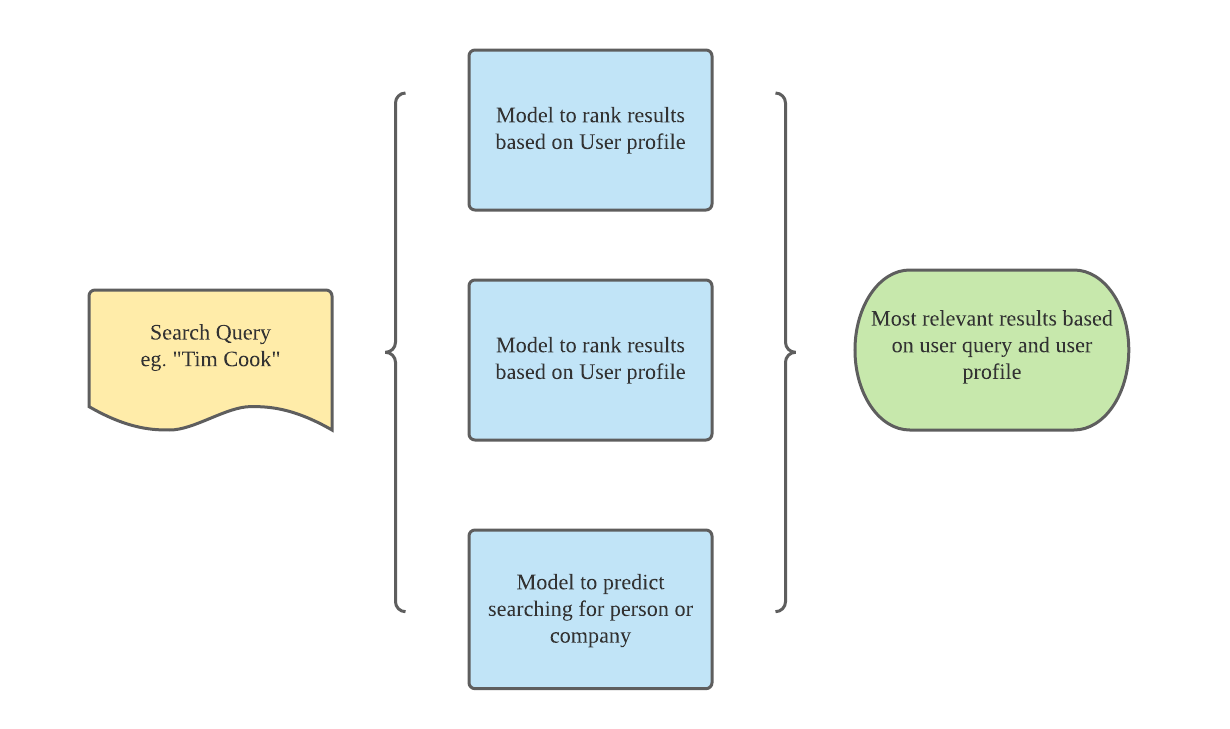
\includegraphics[height=10cm]{jdf-latex/Figures/Prototype 1.png}
	\caption{Use predictive modelling to give the most relevant search results}
	\label{fig:predictive}
\end{figure}

\subsection{Evaluation}
Below are the benefits of using Text(Verbal) Prototypes according to Joyner: (\cite{joyner2016b})

\begin{enumerate}
    \item Revisable during interaction
    \item Disguises superficial details
\end{enumerate}

This interface meets the functionality requires that a user is more likely to find a target comparing to the old interface. Also, it takes little time for a user to learn since it follows the UI of the old interface. It is compatible with both mobile and desktop website as well. Also, it is more efficient than users spend less time to find the target. One missing requirement is that the new interface is not necessarily easier for the user to search. The input search query is the same, people need to know the name to search. This will be addressed in the next design that people can have the search result even without knowing the name.

\section{Prototype 2 - A paper prototype or wireframe}
\subsection{Idea}
Use a photo to do facial recognition and match the LinkedIn profile
\subsection{Prototype}
Prototype is shown in Figure 2 (next page). 
\begin{figure}[h]
	\centering
	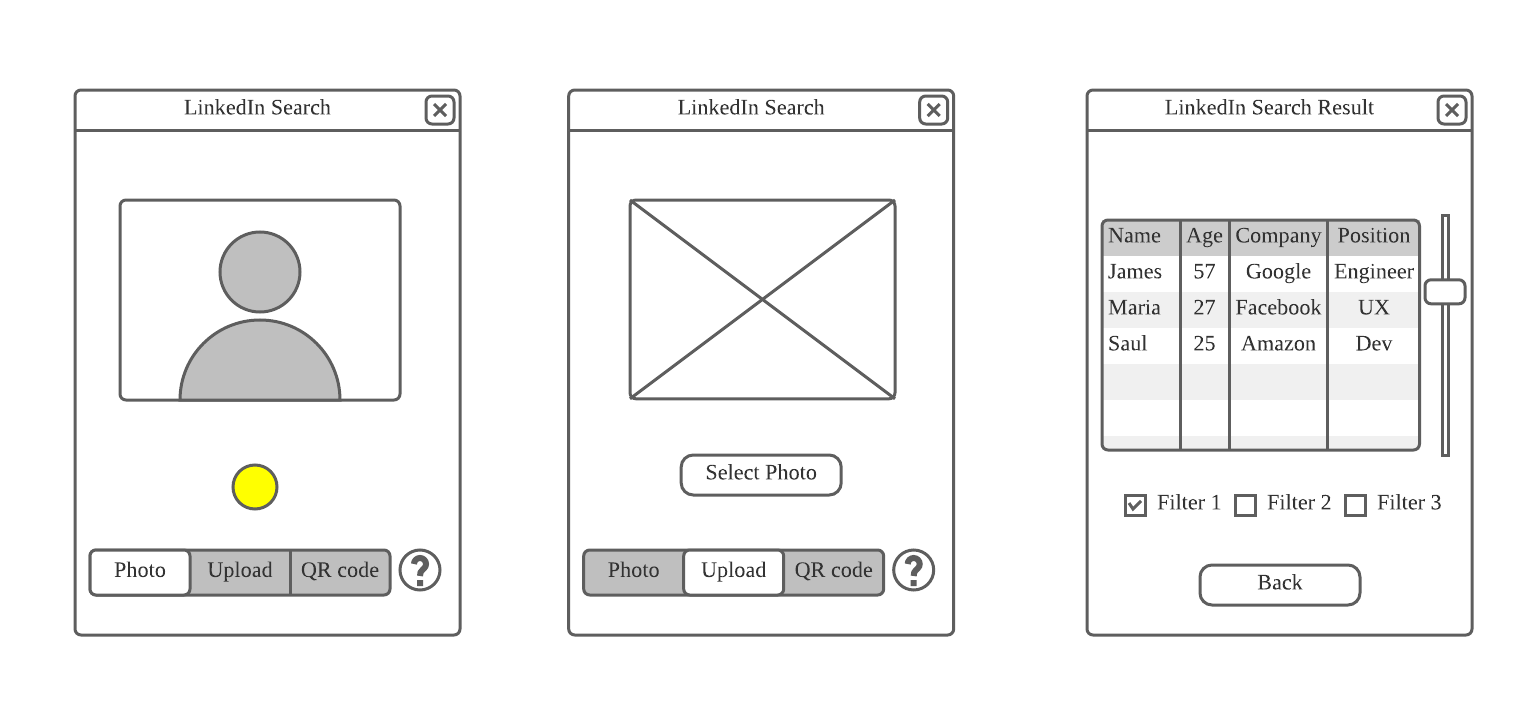
\includegraphics[height=10cm]{jdf-latex/Figures/LinkedIn Search Prototype.png}
	\caption{Wireframe of facial recognition in LinkedIn search function}
	\label{fig:wizard}
\end{figure}
\subsection{Prototype Description}
The interface looks like a camera app. Users can add another user by using the interface to scan the QR code, take a picture of another user to perform facial recognition to find the correct profile or upload a photo to find a target. It can be further utilized to search aged group photos to let one find the LinkedIn profiles of childhood friends. This is one step further that needs an algorithm to match the photo of a person with one from years ago. If the app is uncertain, it will suggest a list of profiles based on the probability of a match. Furthermore, it can have an interface like Google translate that give real-time suggestion next to the current camera view.

The final interface can be a combination of several good ideas from the brainstorming session. In this design, there could be a concern that people may not like to be recognized by the facial recognition, but willing to connect through QR code or Bluetooth. The new interface can have all the options available, but also allow the user to opt-out from certain methods like facial recognition.

\subsection{Evaluation}
Below are the benefits of using Wireframing according to Joyner: (\cite{joyner2016b})

\begin{enumerate}
    \item Simulates user interaction
    \item Easily distributable to remote users
    \item Supports prototyping look and feel
\end{enumerate}

The new interface meets the functionality requirements that people can search a person, even without knowing the name. This is very helpful in the scenarios like welcoming a new joiner but you cannot remember his name. The new interface is also easy to use and learn. It is very efficient as well since all it needs is a photo. It would work both on mobile and desktop website, though on the desktop there is no way to take a photo. Facial recognition is a mature technology and the technology competency is valid, the main concern would be whether this is an ethical AI application.

\section{Prototype 3 - Wizard of Oz}

\subsection{Idea}
Use the voice signature to identify who you are talking with.

\subsection{Description}

\begin{figure}[h]
	\centering
	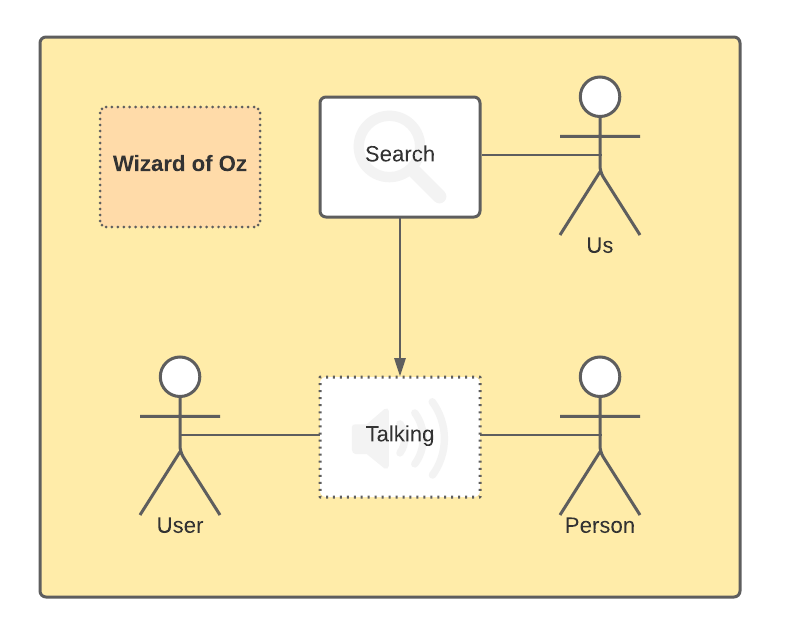
\includegraphics[height=7cm]{jdf-latex/Figures/Wizard of Oz.png}
	\caption{Wizard of Oz prototype for identify who you are talking to}
	\label{fig:wizard}
\end{figure}

When a user is talking to a person, the interface should be able to use the voice signature to identify the person's LinkedIn profile. Here we use the Wizard of Oz prototype to test the user interaction and collect feedback about the interface. When a user is talking to a person in different scenarios, we will search the person's LinkedIn profile, then provide them to user A in the interface. We can even prepare beforehand what is the person's LinkedIn profile before user A talking to the person. The key is to provide this information in the prototype interface while they are talking. Then we can let the user feedback on whether the prototype desirably fulfill the task.

Through the previous needfinding exercises, we know some of the scenarios when people are trying to find out a person's LinkedIn profile. For example, when a new colleague joins the company, one would like to know his background. Another example is when connecting to an old friend, one wants to understand what the friend is currently doing. There are multiple scenarios and we will go through the Wizard of Oz prototype under each of them. Thus we can have a better understanding of how well this new prototype can fulfil the requirements and help people to accomplish the task better.

\subsection{Evaluation}
Below are the benefits of using Wizard of Oz according to Joyner: (\cite{joyner2016b})

\begin{enumerate}
    \item Revisable during interaction
    \item Disguises superficial details
    \item Simulates user interaction
    \item Allows mobility during evaluation
\end{enumerate}


The interface meets functionality requirement, the user can easily find the target. It is very easy to use and almost zero learning effort. It is also very efficient, the result is pushed to the user. It has limited support for the website version. The interface needs voice input unless it is for an online video conference. This is an invisible interface that the user spend zero effort to learn the interface and the result is presented effortlessly. The only concern is that the voice data could be sensitive, it creates an ethical AI application issue.

\section{References}

\printbibliography[heading=none]

\end{document}